\subsection{Spændingsforsyning}
Til systemet anvendes to 9V batterier som spændingsforsyning koblet i et splitsupply. Splitsupply medvirker til at sysemet opnår et arbejdsområde fra $\pm$ 9V. Systemet opsættes så den positive pol på det ene batteri tilkobles den negative pol på det andet batteri, på denne måde opnås en jordforbindelse. Den negative pol i batteri i det første batteri anvendes som systemets negative forsyningsspænding og indikeres med -V_cc, mens det andet batteri anvendes som den positive spændingsforsyning og indikeres med +V_cc. Denne opsætning illustreres på \figref{batteri}. 
Da batterierne ikke leverer den samme spændingsforsyning over batteriernes levetid, skal batteriet skiftes ud når det ikke leverer den spænding som er nødvendig for systemet. Batteriernes levetid afhænger af hvor mange ampere systemet trækker ud. Da feedbacken kræver en spænding på xx V skal systemet minimum leverer en spænding på xx V. Derfor kræver systemt en minimal spænding på xx V.

\begin{figure}[H]
\centering
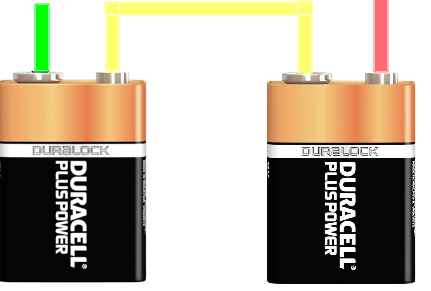
\includegraphics[scale=1]{figures/cProblemloesning/batteri.PNG}
\caption{Figuren viser spændingsforsyningen i et splitsupply, samt hvordan ledningerne mellem de to batterier kobles. Den røde illustrerer +V_cc og den grønne indikere -V_cc}
\label{fig:batteri}
\end{figure}

\subsubsection{Test af spændingsforsyning}
Batteriernes levetid undersøges ved at teste hvor mange ampere systemet bruger. På baggrund af dette vil informationen omkring batteriernes levetid give en estimering af hvornår de skal udskiftes. Testningen foregår ved en serieforbindelse mellem den negative spændingsforsyning- V_cc eller postive spændingsforsyning V_cc og systemet. Selve opsætningen af testen illustreres på \figref{spændingsforsyning}

\begin{figure}[H]
\centering
\includegraphics[scale=1]{figures/cProblemloesning/ltspice.PNG}
\caption{Figuren viser opsætningen af testen af spændingsforsyningen.}
\label{fig:spændingsforsyning}
\end{figure}